% 한국어 검토용 원고. LuaLaTeX으로 빌드한다.
\documentclass[letterpaper,conference]{IEEEtran}

\usepackage{luatexko}
\setmainfont{TeX Gyre Termes}
\setsansfont{TeX Gyre Heros}
\setmonofont{NanumGothicCoding}
\setmainhangulfont{Noto Serif CJK KR}
\setsanshangulfont{Noto Sans CJK KR}
\setmonohangulfont{NanumGothicCoding}
\usepackage{cite}
\usepackage{amsmath,amssymb,amsfonts}
\usepackage{graphicx}
\usepackage{booktabs}
\usepackage{array}
\usepackage{url}
\usepackage{balance}
\usepackage{placeins}

\graphicspath{{./figs/}{./}}
\newcommand{\seTwo}{\mathrm{SE}(2)}
\newcommand{\dchunk}{D_{\mathrm{chunk}}}
\newcommand{\dshape}{D_{\mathrm{shape}}}
\newcolumntype{L}[1]{>{\raggedright\arraybackslash}p{#1}}
\renewcommand{\abstractname}{초록}
\renewcommand{\IEEEkeywordsname}{주요어}
\renewcommand{\figurename}{그림}
\renewcommand{\tablename}{표}
\renewcommand{\refname}{참고문헌}

\begin{document}

\title{언어 조건부 주행을 위한 SmolVLA:\\
일치 입력 및 폐루프 평가}

\author{
\IEEEauthorblockN{Sun Hong Jung}
\IEEEauthorblockA{\textit{전자전기컴퓨터공학과} \\
\textit{성균관대학교}\\
수원, 대한민국 \\
tjsghd7867@g.skku.edu}
\and
\IEEEauthorblockN{Young Hoon Suh}
\IEEEauthorblockA{\textit{전자전기컴퓨터공학과} \\
\textit{성균관대학교}\\
수원, 대한민국 \\
dudgns0407@g.skku.edu}
\and
\IEEEauthorblockN{Hyo Jin Park}
\IEEEauthorblockA{\textit{전자전기컴퓨터공학과} \\
\textit{성균관대학교}\\
수원, 대한민국 \\
phyojin0511@g.skku.edu}
\and
\IEEEauthorblockN{Jae Wook Jeon$^*$}
\IEEEauthorblockA{\textit{전자전기컴퓨터공학과} \\
\textit{성균관대학교}\\
수원, 대한민국 \\
jwjeon@skku.edu}
}

\maketitle

\begin{abstract}
소형 비전--언어--행동(VLA) 모델은 언어 조건부 로봇 제어를 가능하게 하지만,
차량 형태에 적응한 뒤 지시문을 어떻게 활용하는지는 충분히 규명되지 않았다.
본 연구에서는 388개의 작업 문자열과 93,733개 샘플로 구성된 언어 태그 시연
406개를 이용하여 시뮬레이션 폐루프 제어용 SmolVLA를 미세 조정한다. 정책은 전방
RGB 영상, 영어 지시문, 속도, 요 레이트, 그리고 값이 일정한 레거시 상태 슬롯을
30단계 증분형 $\seTwo$ 청크로 매핑한다. 일치 입력 $2^3$ 개입 실험은 고정된 관측
20개에 대해 템플릿, 시험 대상인 \emph{inner/outer}에서
\emph{innermost/outermost}로의 치환, 속도 표현을 변화시킨다. Base 표현의 원시
행동 경로 분리 중앙값은 0.690~m이며, 차선 1 동일 지시문 기준값은 0.125~m이다.
템플릿만 또는 속도 표현만 바꾸었을 때는 각각 0.826~m와 0.672~m가 유지되지만,
시험한 차선 표현 치환은 분리를 0.093~m로 감소시킨다. 이 양상은 오프라인 브리지
변환 후에도 유지된다. 두 시작점과 두 지시 순서를 균형화한 실시간 기준 롤아웃
32회에서 Base의 서로 다른 지시문 쌍은 7.376~m의 궤적 분리 중앙값을 보인 반면,
반복 지시문 기준값은 0.177~m이다. Base 롤아웃 16회에서 15~m 이후 재표본화된
모든 점은 요청 차선에 더 가깝지만, 시험 표현으로 안쪽 차선을 요청한 8회에서는
모든 점이 바깥쪽 기준선에 더 가깝다. 이 결과는 측정 가능한 언어-동작 경로를
입증하고, 관측된 성능 저하가 일반적인 문장 신규성이 아니라 시험한 특정 치환에서
발생했음을 보여준다.
\end{abstract}

\begin{IEEEkeywords}
VLA, SmolVLA, 언어 조건부 주행, 행동 청킹, 폐루프 평가, ROS~2
\end{IEEEkeywords}

\begin{figure*}[!t]
  \centering
  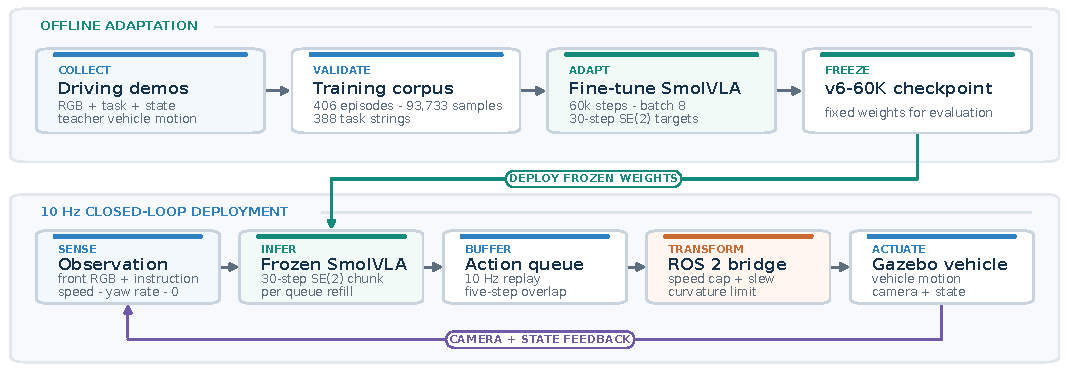
\includegraphics[trim=4.8bp 6.2bp 4.8bp 3.5bp,clip,width=\textwidth]{fig1_language_pipeline.pdf}
  \caption{학습 및 배포 파이프라인. 고정된 SmolVLA는 RGB, 언어, 상태를
  ROS~2--Gazebo에서 10~Hz로 재생되는 30단계 $\seTwo$ 청크로 매핑한다.}
  \label{fig:pipeline}
  \vspace{-7pt}
\end{figure*}

\section{서론}
비전--언어--행동 모델은 자연어, 시각 인식, 연속 로봇 제어를 연결하는 공통
인터페이스를 제공한다. OpenVLA는 공개 사전 학습 VLA를 여러 조작 플랫폼과 작업에
적응할 수 있음을 보였고~\cite{openvla}, SmolVLA는 청크형 연속 행동을 유지하면서
정책 규모를 약 4억 5천만 개 파라미터로 줄였다~\cite{smolvla}. 이 소형 모델은 로봇과
차량 시제품에 유용하지만, 새로운 형태에 적응시킬 때 기본적인 실증 질문이 생긴다.
미세 조정된 정책은 동작을 선택하기 위해 지시문을 사용하는가, 아니면 시각적으로
그럴듯한 경로를 주로 재현하는가?

차량 주행에서는 이 차이를 관찰할 수 있다. 두 차선 지시문은 초기 카메라 영상과
차량 상태가 같더라도 서로 다른 미래 경로를 요구할 수 있다. 언어를 무시하는 정책도
부드럽게 주행할 수 있으므로, 작업 완료나 차선 유지 자체만으로는 언어 조건부 동작을
입증할 수 없다. 반대로 두 확률적 정책 샘플 사이의 차이만으로 지시문 변경이 그 차이를
일으켰다고 볼 수도 없다. 따라서 평가는 시각 및 상태 관측을 고정하고, 생성된 행동
청크를 겹치지 않는 시드의 동일 지시문 기준과 비교하며, 행동이 폐루프에 들어간 뒤에도
분리가 유지되는지 확인해야 한다.

본 연구에서는 언어 태그 시연으로 미세 조정한 시뮬레이션 차량형 플랫폼용 SmolVLA
체크포인트를 분석한다. 정책은 전방 영상 한 장, 영어 문장, 속도, 요 레이트, 값이
일정한 레거시 상태 슬롯을 입력받아 30개의 증분형 자차 운동 행동을 예측한다. 정책은
Gazebo의 ROS~2 브리지를 통해 배포되며, 브리지는 체크포인트 출력을 동작 명령으로
결정론적으로 변환한다. 광범위한 자연어 이해를 주장하는 대신, 관찰된 구성요소로 만든
Base 표현과 차량 미세 조정 목록에 없는 문구 은행 구성요소로 만든 대칭적인 시험 표현
쌍을 비교한다. 완성된 평가 문장 16개 중 복구된 최종 작업 목록에 그대로 존재하는
문장은 없다. 세 표현 구성요소를 요인별로 변화시켜 차선 반응 손실과 관련된 시험
변경을 식별한다.

본 연구의 기여는 다음 세 가지이다.
\begin{enumerate}
    \item 검증된 시연부터 30단계 증분형 $\seTwo$ 청크와 ROS~2--Gazebo 실행까지
    포함하는 언어 조건부 차량 제어용 소형 VLA 적응 파이프라인,
    \item 템플릿, 시험 대상인 \emph{inner/outer}에서
    \emph{innermost/outermost}로의 치환, 속도 표현의 효과를 분리하고 원시 경로와
    오프라인 브리지 변환 민감도 경로를 모두 확인하는 일치 관측 $2^3$ 개입 실험,
    \item 기본 언어 구분이 차량 실행에서도 유지됨을 보이는 균형화된 폐루프 롤아웃
    32회와 시험한 치환에서 관찰된 폐루프 실패이다.
\end{enumerate}

\section{관련 연구}
OpenVLA는 공개형 다운스트림 VLA 적응을 확립했으며, SmolVLA는 소형 백본과 플로
매칭 행동 청크를 결합한다~\cite{openvla,smolvla}. ROS2SmolVLA는 ROS~2를 통해
SmolVLA를 산업용 매니퓰레이터와 통합한다~\cite{ros2smolvla}. 반면 본 연구의 형태와
평가는 평면 차량 제어와 주행 지시문의 측정된 효과를 다룬다.

본 연구실의 축소형 차량 연구 계보에서 Oh \emph{et al.}은 경진대회 기반 자율주행
교육 프레임워크를 개발했고~\cite{oh2026education}, Hong \emph{et al.}은 규칙 기반
제어와 학습형 종단간 차량 제어를 비교했다~\cite{hong2025datadriven}. Suh
\emph{et al.}은 모듈형 검출기--VLM 주행 스택~\cite{suh2025modularvla}과 이후
지연 인식형 저속/고속 안전 중재 구조~\cite{suh2026lasa}를 평가했다. 이 연구들은
본 연구의 플랫폼, 학습, VLA 계보를 형성한다. 본 연구는 이 계보의 시뮬레이션 트랙과
고정된 안쪽/바깥쪽 차선 식별자를 재사용하지만, 각 에피소드 지시문은 하나의 차선 변경
명령 대신 차선, 속도 표현, 그리고 대개 목적지나 정지 목표를 함께 지정한다.

SimLingo는 언어 정렬 폐루프 주행을 연구하고, OpenDriveVLA는 인식, 상태, 운전자
명령으로 궤적을 예측한다~\cite{simlingo,opendrivevla}. LinkVLA는 언어--행동 정렬을
직접 학습하며~\cite{linkvla}, ICR-Drive는 통제된 텍스트 변경으로 지시문의 효과를
분리한다~\cite{icrdrive}. 조작 벤치마크에서도 같은 유형의 실패가 보고된다. 시각적으로
그럴듯한 배치에서 반사실적 지시문을 할당하면 시각 지름길이 드러나며~\cite{liberocf},
동의어 수준의 바꿔쓰기만으로도 작업 성공률이 낮아진다~\cite{liberopara}. 따라서 본
연구는 실패 양상 자체가 새롭다고 주장하지 않는다. 기존 평가와 달리, 차량 정책의
요인화된 행동 청크 개입에서 정확히 같은 RGB/상태 입력을 고정하고, 측정된 차이가
ROS~2--Gazebo 폐루프 실행기를 통과한 뒤에도 유지되는지 시험한다.

\section{방법론}
그림~\ref{fig:pipeline}은 전체 시스템을 요약하고, 표~\ref{tab:configuration}은 학습
및 배포 구성을 제시한다. 학습 구성요소는 미세 조정된 SmolVLA 정책이며, 보고한 모든
평가에서 같은 고정 체크포인트를 사용한다.

\subsection{시연 말뭉치}
교사 제어기는 링 주행 동작을 생성하고, 에피소드 단위 영어 지시문은 차선과 속도,
그리고 흔히 랜드마크 목적지나 정지 작업을 지정했다. 각 원시 에피소드는 30~Hz의
전방 카메라 스트림, 언어 레이블, 차량 상태, 교사 제어, 전역 자세를 포함했다. 검증
단계에서 불완전하거나 기하학적으로 유효하지 않은 에피소드를 제외하고, 유지된 기록은
10~Hz LeRobot 형식으로 재표본화했다. 최종 v6 LeRobot 메타데이터에는 에피소드
406개, 행동 행 93,733개, 고유 작업 문자열 388개가 기록되어 있다. 이 문자열은 이름이
있는 트랙 목표 여섯 개와 한 바퀴 주행 형식에 대해 바꿔 쓴 표면형으로 차선, 속도,
목적지 슬롯을 조합한다. 이러한 조합은 후속 시험의 전제가 된다. 차선은 세 슬롯 중
하나이므로 차선 의존 반응은 두 개의 고정 문자열 일치에서 나올 수 없으며, 템플릿과
속도 슬롯이 나머지 두 표현 요인을 제공한다. 학습 산출물에서 전체 작업 목록을 복구해
정렬된 해시와 함께 평가 기록에 저장했다.

체크포인트의 3차원 상태는 다음과 같다.
\begin{equation}
\mathbf{s}_t=[v_t,\dot{\psi}_t,0],
\label{eq:state}
\end{equation}
여기서 $v_t$와 $\dot{\psi}_t$는 각각 차량 속도와 요 레이트이다. 세 번째 레거시 상태
슬롯은 학습 행 93,733개 모두에서 항상 0이며, 평가에서도 0으로 강제된다. 이 값은
측정된 조향 신호로 취급하지 않는다. 전역 위치와 지도 좌표는 정책 입력에서 제외한다.
학습 목표는 0.1초 한 단계 동안의 자차 좌표계 변위
$\mathbf{a}_i=[\Delta x_i,\Delta y_i,\Delta\psi_i]$이다. 따라서 초기 시각 및 상태
관측이 같을 때 정책이 따라야 할 차선을 직접 지정하는 입력은 언어뿐이다.

\subsection{정책 및 미세 조정}
소형 SmolVLA 릴리스에서 시작하여 다음을 예측하는 정책을 미세 조정한다.
\begin{equation}
\mathbf{A}_t=\pi_\theta(I_t,\ell,\mathbf{s}_t),\qquad
\mathbf{A}_t\in\mathbb{R}^{30\times3},
\label{eq:policy}
\end{equation}
여기서 $I_t$는 전방 RGB 영상이고 $\ell$은 영어 작업 지시문이다. 학습은 배치 크기 8,
학습률 $10^{-4}$, 자동 혼합 정밀도, 시드 1000, 영상 증강 없음의 조건으로 최적화
60,000단계 동안 수행한다. 이는 93,733개 행 말뭉치를 약 5.12회 순회한 것에 해당한다.
생성된 v6-60K 체크포인트는 모든 실험에서 고정한다.

체크포인트는 SmolVLA의 SmolVLM2-500M-Video-Instruct 백본, 교차 어텐션 행동 조건화,
플로 매칭 잡음 제거 10단계를 유지한다. AdamW, 1,000단계 워밍업, 코사인 감쇠를
사용해 전체 정책을 갱신하며, 모든 설정은 언어 조건 간 동일하게 유지한다.

분석을 위해 예측 증분을 자차 좌표계 경로로 합성한다.
\begin{equation}
\mathbf{p}_0=\mathbf{0},\qquad
\mathbf{p}_{i+1}=\mathbf{p}_i\oplus\mathbf{a}_i,\quad i=0,\ldots,29,
\label{eq:compose}
\end{equation}
여기서 $\oplus$는 누적 요 각도로 병진 변위를 회전한 뒤 적용한다. 이는 $\Delta y$를
포함한 \emph{원시} 정책 출력으로 합성한 진단 경로이며, 시뮬레이션 차량 궤적이 아니다.
아래와 같이 배포 재생에서는 $\Delta x$와 $\Delta\psi$를 사용하며, 폐루프 평가는 그에
따른 실제 차량 동작을 측정한다.

\begin{table}[!ht]
\caption{학습 및 배포 구성}
\label{tab:configuration}
\centering
\footnotesize
\setlength{\tabcolsep}{3.0pt}
\begin{tabular}{@{}L{0.25\columnwidth}L{0.67\columnwidth}@{}}
\toprule
항목 & 구성 \\
\midrule
정책 & SmolVLA, 약 4억 5천만 파라미터, 고정된 v6-60K 체크포인트 \\
말뭉치 & 에피소드 406개, 10~Hz 기준 93,733행, 작업 문자열 388개 \\
관측 & 전방 RGB, 영어 작업, 속도, 요 레이트, 항상 0인 레거시 슬롯 \\
행동 & 0.1초 간격의 $30\times[\Delta x,\Delta y,\Delta\psi]$ \\
미세 조정 & 60K 단계, 배치 8, 학습률 $10^{-4}$, AMP, 시드 1000, 영상 증강 없음 \\
큐 & 10~Hz, 5단계 중첩, 30\% 잔여 시 보충, 직접 재생 \\
명령 한계 & 속도 2.25~m/s, 슬루율 0.08~m/s/tick, 곡률 0.239~m$^{-1}$ \\
평가 & 링 1개, 일치 시작점 2개, 실시간 30초 실행, 정책 시드 0 \\
\bottomrule
\end{tabular}
\end{table}

\subsection{ROS~2--Gazebo 배포}
ROS~2 배포 시스템~\cite{ros2}은 영상, 상태, 래치된 작업을 정책 서버로 보내고 30단계
행동 청크를 수신한다. 브리지는 5단계 중첩 큐를 유지하며 30\%가 남으면 새 청크를
요청한다. 10~Hz의 각 틱에서 직접 재생은 다음 원시 속도와 곡률을 얻는다.
\begin{equation}
v_i^{0}=\frac{\Delta x_i}{0.1},\qquad
\kappa_i^{0}=\frac{\Delta\psi_i}{\Delta x_i}\quad(|\Delta x_i|>10^{-4}\ \mathrm{m}),
\label{eq:replay}
\end{equation}
그런 다음 속도를 2.25~m/s로 제한하고, 틱당 변화량을 0.08~m/s로 제한하며,
$\kappa_i^0$를 $\pm0.239$~m$^{-1}$로 클리핑한 뒤 $\omega_i=\kappa_i v_i$를
발행한다. $|\Delta x_i|\le10^{-4}$~m일 때는 원시 요 레이트를 대신 유지한다. 횡방향
예측 $\Delta y_i$는 실행기로 보내지 않는다. Gazebo는 차동 구동 플러그인으로 몸체가
움직이는 차량형 모델을 중심으로 카메라와 상태 루프를 닫는다~\cite{gazebo}. 앞바퀴
조향 관절은 해당 곡률을 시각화하지만 몸체 동역학을 정의하지 않는다. 지도, 목표 벡터,
전역 자세는 정책에 전달하지 않는다.

서버는 전방 영상 하나를 감지하고, 체크포인트에서 카메라 키를 가져오며, 저장된
정규화기에서 실제 3차원 상태 폭을 복구한다. 상속된 미사용 카메라 슬롯과 기본 구성의
자리 표시용 6차원 상태 형상은 무시한다.

평가 시 각 일치 명령 자세 초기화 후 시뮬레이터를 일시 정지하고 지시문을 발행하며,
첫 행동 청크가 도착한 뒤에만 실행을 시작한다. 이 사전 채움 프로토콜은 시작 지연이
제어기 워치독 실패로 집계되는 것을 막으며, 예측 행동이나 이후 폐루프 제어는 변경하지
않는다. 명령 위치가 5~cm 이내로 확인되고 궤적에 보존된 점이 5개 이상이며, 워치독
활성화와 행동 언더런이 모두 0인 경우에만 롤아웃을 채택한다.

\subsection{평가 프로토콜}
\subsubsection{일치 관측 행동 시험}
v6 학습 계보의 세 수집 세션에서 검증된 차선 반사실 그룹 20개를 표본화하고, 공통
시작 후 명목상 0.5초에 해당하는 10~Hz 행 인덱스 5를 선택한다. 각 그룹에서 정확히
같은 RGB 배열과 상태 벡터를 양쪽에 입력하고 지시문만 바꾼다. $2^3$ 설계는 세 가지
이진 표현 구성요소를 변경한다. 템플릿 $T$ (``Start driving''/``Roam the track''),
차선 치환 $L$ (``inner, outer''/``innermost, outermost''), 속도 표현 $S$
(``normal''/``regular'')이다. 차선 의미는 바꾸지 않은 채 Base, $T$, $L$, $S$,
$T{+}L$, $T{+}S$, $L{+}S$, $T{+}L{+}S$ 셀을 구성한다.

완성된 평가 문장 16개 중 복구한 388개 작업 학습 목록에 그대로 등장하는 문장은 없다.
Base 구성요소는 목록에 있지만, 대체 $T$, $L$, $S$ 구성요소는 모두 0회 등장하며 v6
학습 전에 커밋된 문구 은행에 속한다. 따라서 이 설계는 고정된 표현 집합 안에서 반응을
국소화한다. 시각 관측 자체는 홀드아웃이 아니다.

SmolVLA 표본화에는 확률성이 있다. 시드 0--3을 사용해 각 지시문의 예측 청크 4개를
평균한다. 참고를 위해 같은 영상, 상태, 차선 1 문장을 겹치지 않는 시드 4--7로 다시
표본화한다. 이는 비대칭 차선 1 동일 지시문 기준이며 두 지시문의 확률적 변동에 대한
상한이 아니다. $P_{xy}(\ell)=\{\mathbf{p}_{i,xy}(\ell)\}_{i=1}^{30}$가
식~\eqref{eq:compose}의 원시 합성 자세 중 병진 성분을 포함한다고 하자. 지시문 분리는
다음과 같다.
\begin{equation}
\dchunk(\ell_1,\ell_2)=
\sqrt{\frac{1}{30}\sum_{i=1}^{30}
\left\|\mathbf{p}_{i,xy}(\ell_1)-\mathbf{p}_{i,xy}(\ell_2)\right\|_2^2}.
\label{eq:dchunk}
\end{equation}
각 관측에 대해 $R=\dchunk/D_{\mathrm{ref},1}$도 보고한다. 여기서
$D_{\mathrm{ref},1}$은 겹치지 않는 시드의 차선 1 청크에 식~\eqref{eq:dchunk}를
적용한 값이며, $R>1$이면 이 범위로 한정한 동일 지시문 기준을 넘는다. 요인 효과는 각
관측 안에서 계산한 $\log_2(\dchunk/1\,\mathrm{m})$의 포화 대비이며, 50,000회 재표본
쌍체 부트스트랩으로 요약한다. 구간은 이 고정 표본에 대한 탐색적 점별 구간이다.

저장된 4개 시드 평균 청크는 초기 명령이 0인 브리지 변환 민감도 확인에도 사용한다.
관측 속도는 0.562--2.181~m/s 범위이지만, 이 진단에서는 \emph{이전 명령} 속도를 0으로
초기화하고 $\Delta y$를 제거한다. 또한 기록된 속도 상한과 슬루 제한, 식~\eqref{eq:replay}에
정의된 곡률 클리핑을 적용하고, 결과 유니사이클 명령을 적분해 분리를 다시 계산한다.
큐 보충, 이어 붙이기, Gazebo는 모사하지 않으며, 이러한 효과는 폐루프 실행에서만 평가한다.

\subsubsection{쌍체 폐루프 시험}
폐루프에서는 요인 설계의 두 끝점인 Base와 $T{+}L{+}S$만 평가한다. 개별 요인의
국소화는 행동 수준에서만 수행한다. 트랙의 같은 종방향 인덱스에서 안쪽 차선과 바깥쪽
차선 시작점을 사용한다. 표현 조건 및 시작점별로 한 번은 안쪽 다음 바깥쪽(AB), 다른
한 번은 바깥쪽 다음 안쪽(BA) 순서로 실행한다. 각 호출은 동일 지시문 쌍 $(A,A)$를
기록한 뒤 서로 다른 지시문 쌍 $(A,B)$을 기록한다. 따라서 각 시작점에서 동일 안쪽과
동일 바깥쪽 기준 및 두 지시 순서를 모두 관찰한다. 물리 롤아웃 수는 $2$개 표현 조건
$\times2$개 시작점 $\times2$개 순서 $\times4$회로 총 32회이다. 각 실행은 정책 시드
0으로 실시간 30초 동안 수행한다.

공간적으로 솎은 궤적은 공통 이동 길이로 잘라내며, 이산 Fr\'{e}chet 거리를
$\dshape$로 보고한다. 이 척도는 궤적 순서를 고려하면서 경로 분리를 측정한다. 공통
접두 길이는 재표본화 경로 사이의 차이가 처음으로 0.30~m를 넘기 전까지 이동한
거리이다. 두 값 모두 행동 차별화 척도이며, 그 자체로 올바른 차선 점유나 안전 주행을
입증하지는 않는다.

방향성 확인을 추가하기 위해 공통 시작과 차선 전환이 결과를 지배하지 않도록 각 궤적의
첫 15~m를 제외한다. 남은 각 점 $\mathbf{x}$에 대해 구성된 두 차선 중심선 폴리라인
$R_1$, $R_2$까지의 유클리드 거리를 계산한다. 차선 $\ell$을 요청하는 지시문의 경우
실행별 중앙값과 95백분위수를 다음과 같이 보고한다.
\begin{equation}
d_\ell(\mathbf{x})=\min_{\mathbf{r}\in R_\ell}
\|\mathbf{x}-\mathbf{r}\|_2,
\label{eq:lane_distance}
\end{equation}
구현은 표본 정점만이 아니라 선분 위로 투영한다. 또한 분석한 점 중
$d_\ell(\mathbf{x})<d_{3-\ell}(\mathbf{x})$인 비율을 보고한다. 이는 중심선 상대 경로
검사이며, 차선 경계나 충돌 안전성 척도가 아니다.

\subsubsection{재현성 및 타당성 통제}
독립적인 SHA-256 검사를 통해 폐루프와 오프라인 평가가 같은 체크포인트를 사용했음을
확인하며, 전체 다이제스트는 체크포인트 매니페스트에 보존한다. 복구된 학습 목록과
해시, 관측 식별자 및 상태 벡터 20개, 원시 평균 청크, 시드별 프로토콜, 전체 폐루프 XY
추적값, 정확한 문자열, 초기화 좌표, 고유 롤아웃 ID, 적용된 브리지 계약, 지연 시간,
워치독 횟수, 언더런 비율을 프로젝트 평가 기록에 보존한다. 정책이나 시뮬레이터를
호출하지 않고 그림과 표 값을 재생성한다. 빈 작업은 배포된 브리지를 해제하므로 빈
언어 대조군은 보고하지 않는다.

\section{결과}
\subsection{행동 청크의 지시문 조건화}
그림~\ref{fig:chunks}은 각 표현 셀에서 관측 수준의 언어/기준 비율 20개를 모두
표시하고, 표~\ref{tab:chunks}은 정확한 요약값을 제시한다. $L$이 없을 때 $R$ 중앙값은
5.14--6.15이며 모든 셀이 20/20개 관측에서 기준을 초과한다. \emph{inner/outer}를
\emph{innermost/outermost}로 바꾸는 시험 치환($L$)을 적용하면 $R$ 중앙값은
0.42--0.52로 떨어지고 20개 중 0--1개만 기준을 초과한다. 원시 $\dchunk$도 $L$이
없을 때 0.672--0.826~m, 있을 때 0.062--0.093~m로 구분된다.

\begin{figure}[!ht]
  \centering
  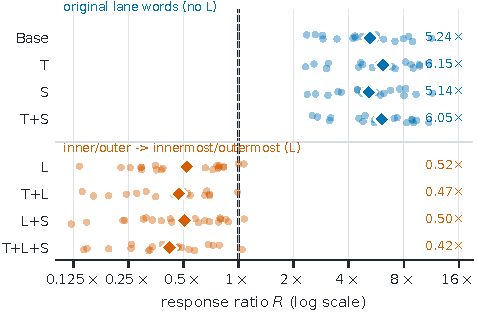
\includegraphics[width=0.99\columnwidth]{fig3_wording_factorial.pdf}
  \caption{8개 표현 셀의 원시 반응 비율 $R$. 작은 점은 일치 관측 20개이고 마름모는
  중앙값이다. $R=1$(점선)은 겹치지 않는 시드의 차선 1 동일 지시문 기준과 같다.
  $T$, $L$, $S$는 각각 템플릿, 시험한 차선 치환, 속도 표현을 뜻한다.}
  \label{fig:chunks}
\end{figure}

\begin{table}[!ht]
\caption{$2^3$ 일치 관측 원시 행동 분리}
\label{tab:chunks}
\centering
\footnotesize
\setlength{\tabcolsep}{3.0pt}
\begin{tabular}{@{}lcccc@{}}
\toprule
셀$^a$ & \shortstack{$\dchunk$\\언어 (m)} & \shortstack{차선 1\\기준 (m)} & \shortstack{중앙값\\비율$^b$} & \shortstack{기준\\초과} \\
\midrule
Base & 0.690 & 0.125 & 5.24 & 20/20 \\
$T$ & 0.826 & 0.123 & 6.15 & 20/20 \\
$S$ & 0.672 & 0.121 & 5.14 & 20/20 \\
$T{+}S$ & 0.823 & 0.123 & 6.05 & 20/20 \\
$L$ & 0.093 & 0.250 & 0.52 & 1/20 \\
$T{+}L$ & 0.062 & 0.205 & 0.47 & 0/20 \\
$L{+}S$ & 0.090 & 0.218 & 0.50 & 1/20 \\
$T{+}L{+}S$ & 0.063 & 0.220 & 0.42 & 1/20 \\
\bottomrule
\multicolumn{5}{@{}l}{\scriptsize $^aT$: 템플릿, $L$: 시험한 차선 치환, $S$: 속도 표현.}\\[-1pt]
\multicolumn{5}{@{}l}{\scriptsize $^b$관측별 언어/기준 비율의 중앙값.}
\end{tabular}
\end{table}

별도로 원시 $\dchunk$ 요인 대비에서 $\log_2(\dchunk/1\,\mathrm{m})$에 대한 $L$의
효과는 $-3.118$이며, 쌍체 부트스트랩 95\% 구간은 $[-3.469,-2.797]$이다. 이는 요인
기하 평균 배율 0.115에 해당한다. 배율 척도에서 $T$ 주효과와 $T{\times}L$ 상호작용은
각각 0.916 $[0.852,0.984]$와 0.828 $[0.769,0.890]$이다. $S$와 나머지 상호작용의
로그 척도 구간은 0을 포함한다. 따라서 이 고정 오프라인 표현 개입에서 $L$은 지배적이나
유일하지는 않은 음의 요인이다.

초기 명령이 0인 브리지 변환 검사에서도 같은 지배 요인이 나타난다. $L=-3.339$
$[-3.704,-3.009]$이고 기하 평균 배율은 0.099이다. Base와 $T{+}L{+}S$의 중앙값은
각 차선 1 기준과 비교할 때 각각 0.221 대 0.031~m, 0.016 대 0.037~m이다. 8개 셀
모두 원시 경로와 변환 경로에서 기준 상회/하회 중앙값 분류가 동일하게 유지된다.

\begin{figure*}[!t]
  \centering
  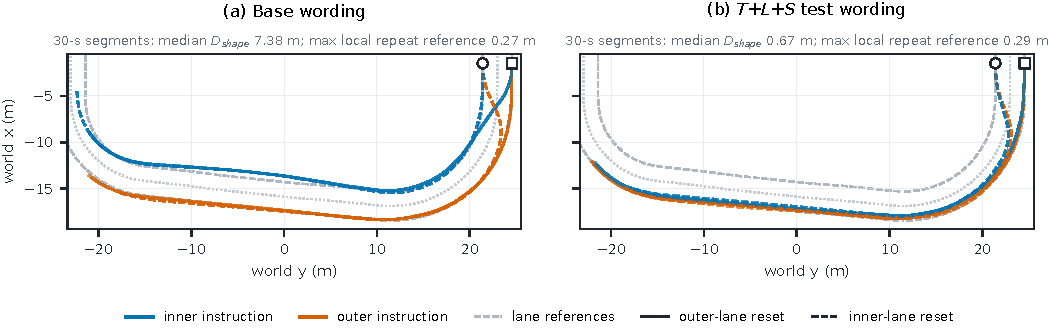
\includegraphics[width=0.985\textwidth]{fig2_closed_loop_language.pdf}
  \caption{일치 초기화에서 수행한 실시간 30초 폐루프 구간. 색은 요청 차선, 선 종류는
  초기화 차선을 나타내고 회색 곡선은 차선 기준선이다. Base 표현은 두 경로를 모두
  선택하지만 $T{+}L{+}S$ 시험 표현은 바깥쪽 경로로 수렴한다.}
  \label{fig:closedloop}
\end{figure*}

\subsection{폐루프 언어 반응}
그림~\ref{fig:closedloop}과 표~\ref{tab:closedloop}의 폐루프 결과는 행동 수준 시험에
방향성 정보를 보완한다. Base 표현은 서로 다른 지시문 쌍 4개에서
$\dshape=7.376$~m를 보이는 반면, 동일 지시문 쌍 4개의 중앙값은 0.177~m이다. 서로
다른 네 쌍은 모두 각 초기화의 동일 안쪽 및 동일 바깥쪽 값 중 큰 값으로 정의한 국소
반복 지시문 기준을 초과한다. 두 시작점과 AB/BA 두 순서에서 모두 결과가 유지되며,
최초로 $>0.30$~m 차이가 나는 시점은 이동 거리 중앙값 2.5~m 이후이다.

\begin{table}[!ht]
\caption{쌍체 폐루프 궤적 분리}
\label{tab:closedloop}
\centering
\footnotesize
\setlength{\tabcolsep}{0.6pt}
\begin{tabular}{@{}lcccc@{}}
\toprule
표현 & \shortstack{상이 $\dshape$\\중앙값 [범위] (m)} & \shortstack{동일 $\dshape$\\중앙값 [범위] (m)} & \shortstack{국소 기준\\초과} & \shortstack{공통 접두\\길이 (m)} \\
\midrule
Base & 7.376 [6.740, 7.860] & 0.177 [0.167, 0.265] & 4/4 & 2.5 \\
$T{+}L{+}S$ & 0.666 [0.569, 0.889] & 0.243 [0.173, 0.292] & 4/4 & 10.3 \\
\bottomrule
\end{tabular}
\end{table}

표~\ref{tab:adherence}는 분리가 요청한 방향으로 발생했는지 확인한다. 15~m 이후 Base
표현 롤아웃 16회의 모든 표본점은 요청 기준선에 더 가깝다. 목표별 8회 롤아웃에서
실행별 오프셋 중앙값들의 중앙값은 안쪽 0.339~m, 바깥쪽 0.086~m이고, 해당 실행별
95백분위수들의 중앙값은 각각 0.728~m와 0.277~m이다.

\begin{table}[!ht]
\caption{15~m 이후 실행별 중심선 추종도(목표당 8회)}
\label{tab:adherence}
\centering
\footnotesize
\setlength{\tabcolsep}{3.1pt}
\begin{tabular}{@{}llccc@{}}
\toprule
표현 & 요청 & \shortstack{실행 중앙값의\\중앙값 (m)} & \shortstack{실행 P95의\\중앙값 (m)} & \shortstack{실행 비율\\중앙값 (\%)} \\
\midrule
Base & 안쪽 & 0.339 & 0.728 & 100 \\
Base & 바깥쪽 & 0.086 & 0.277 & 100 \\
$T{+}L{+}S$ & 안쪽 & 2.779 & 3.019 & 0 \\
$T{+}L{+}S$ & 바깥쪽 & 0.159 & 0.303 & 100 \\
\bottomrule
\end{tabular}
\end{table}

$T{+}L{+}S$ 표현에서 서로 다른 지시문의 중앙값은 0.666~m, 동일 지시문의 중앙값은
0.243~m이며 공통 접두 길이는 10.3~m로 증가한다. 서로 다른 네 쌍이 모두 국소 기준을
초과하지만, 분리만으로 정확성을 의미하지는 않는다. 안쪽 요청 롤아웃 8회에서 15~m
이후 0.2~m 간격으로 재표본화한 모든 점은 \emph{바깥쪽} 기준선에 더 가깝고, 바깥쪽
요청 롤아웃 8회의 해당 점도 모두 바깥쪽 기준선에 더 가깝다. 같은 0\%/100\% 목표
분할은 10, 15, 20~m 절단점과 두 초기화 차선에서 모두 유지된다. Base의 차선 유지 및
변경 기동은 각각 목표에 더 가까운 비율의 중앙값이 1.0이다. $T{+}L{+}S$에서는 요청
기동이 아니라 바깥쪽 차선 편향에 따라 동작하므로 두 기동 모두 0.5이다.

32회 롤아웃은 모두 기록된 실행 계약을 만족한다. 워치독 발생과 행동 언더런은 0이고,
조향 상태 소스는 항상 0이며, 적용된 속도 상한은 2.25~m/s이다. 첫 청크 사전 채움은
0.239--0.299초이고 브리지 요청 왕복 시간의 실행 평균은 242.1--251.4~ms이다. 궤적은
실시간 30초 동안 52.74--58.98~m를 이동하며, 한 바퀴가 아니라 명목 중심선 길이
141.97~m의 약 0.37--0.42에 해당한다.

\subsection{범위 및 차별점 논의}
결합 시험은 두 인터페이스에서 근거를 제공한다. 정책 인터페이스에서는 같은 인식과
상태에서 Base의 inner/outer 표현이 30단계 동작 예측을 변경한다. 형태 인터페이스에서는
반복 인식, 큐 보충, 차량 동역학이 루프를 닫은 뒤에도 같은 차이가 크게 유지된다. 이
결과는 평가한 시뮬레이터에서 미세 조정된 소형 VLA로 언어 조건부 제어가 가능함을
보이며, 다른 정책과의 비교를 의미하지 않는다.

시험 표현의 결과는 해당 문구 쌍에 한정된다. 이 고정 요인 집합에서
\emph{inner/outer}를 유지하는 조합만 강건한 차선 의존 행동 변화를 보인다. 시험한
\emph{innermost/outermost} 치환만으로 보지 못한 차선 표현 전반에 대한 실패를 확정할
수 없다. 완성된 평가 문장 16개가 작업 목록에 하나도 없으므로, 정확한 문자열의
신규성은 언어 일반화의 충분한 근거가 아니다. 차량 VLA 평가는 표현 구성요소를
요인화하고, 각 반응을 범위가 명확한 동일 지시문 기준과 비교해야 한다.

본 연구는 새로운 VLA 구조나 행동 청크 실행기를 제안하지 않는다. 기여는 형태와 평가
방법론에 있다. 행동 수준 일치 입력 시험은 시각적으로 그럴듯한 주행을 언어 사용으로
오인하는 것을 막고, 쌍체 폐루프 시험은 측정된 조건화가 시뮬레이션 차량 궤적에 영향을
줄 만큼 큰지 판단한다.

\subsection{타당성 위협}
실험은 시뮬레이터 트랙 1개, 일치 시작점 2개, 차선 의도 2개, 영어 지시문, 차량
스냅샷 1개, 미세 조정 체크포인트 1개를 사용한다. 속도와 목적지 슬롯은 의미상 고정되어
있으므로 그 조건화에 대해서는 주장하지 않는다. 폐루프 시험 32회는 정책 시드 0으로
순차 실행한 것이며 독립적인 학습 또는 시뮬레이터 시드가 아니므로 유의성 주장을 하지
않는다. AB/BA는 지시 순서를 균형화하지만, 각 호출에서 SAME은 항상 DIFFERENT보다
먼저 실행된다. 초기화 위치는 5~cm 이내인지 확인하지만, 요 값은 기록만 하고 채택 허용
오차로 사용하지 않는다. 일치 관측 20개는 학습 계보의 세 수집 세션에서 얻었으므로,
고정 영상에 대한 조건화 개입을 시험할 뿐 시각 또는 장면 일반화를 시험하지 않는다.
대칭 시험 표현 쌍은 탐색적 오프라인 조사 후 선택되었다. 따라서 요인 및 폐루프 결과는
알려진 실패를 특성화하며, 바꿔쓰기 성공률에 대한 비편향 추정치가 아니다. 점별
부트스트랩은 일치 관측 20개를 재표본 단위로 취급하며, 수집 세션 군집화, 체크포인트
학습 불확실성, 추가 정책 표본화 불확실성을 모델링하지 않는다. 롤아웃은 실시간 30초
구간을 사용하지만 제어 타이머는 ROS/Gazebo 시뮬레이션 시간을 따른다. 시뮬레이터
실시간 계수와 경과 시뮬레이션 시간은 저장하지 않았다. 따라서 보고한 거리와 실시간은
표준화된 시뮬레이션 시간 속도 벤치마크가 아니다.

적응하지 않은 SmolVLA 체크포인트에는 호환되는 차량 행동 정규화기가 없으므로 수치형
사전 학습 정책 기준을 보고하지 않으며, 미세 조정이 기존 주행 점수를 향상시킨다고
주장하지 않는다. 마찬가지로 $\dchunk$와 $\dshape$는 경로 정확성, 차선 경계 여유,
승차감, 안전이 아니라 분리를 측정한다. 교통, 장애물, 날씨, 센서 고장, 실제 차량,
기능 안전 특성은 평가하지 않는다. 차량형 시뮬레이터는 차동 구동 몸체 동역학을
사용하며, 보이는 앞바퀴 조향은 Ackermann 또는 실제 자동차 동역학 검증이 아니다.
더 넓은 결론을 위해서는 여러 지도와 시작점, 독립적으로 학습한 체크포인트, 표현 차이를
단계화한 바꿔쓰기 집합, 그리고 본 연구의 통제 조건화 시험에 더해 목표 또는 차선 정확도
척도가 필요하다.

\balance
\section{결론}
소형 SmolVLA가 전방 영상, 영어 주행 지시문, 체크포인트에 맞춘 상태를 30단계 증분형
$\seTwo$ 행동 청크로 매핑하도록 미세 조정하고, ROS~2--Gazebo 루프에 배포했다.
오프라인 일치 입력 $2^3$ 개입 실험에서 차선 조건부 행동 분리 손실의 지배 요인은
\emph{inner/outer}를 \emph{innermost/outermost}로 치환한 것이었으며, 이 결론은
브리지 변환 검사에서도 유지되었다. 두 시작점과 두 지시 순서에서 Base 폐루프 분리는
7.376~m, 동일 지시문 기준은 0.177~m였다. Base 롤아웃 16회에서 15~m 이후 0.2~m
간격으로 재표본화한 모든 점은 요청 기준선에 더 가까웠다. 보존된 롤아웃 32회 모두
워치독 발생과 행동 언더런이 0이었다. 시험 표현으로 안쪽 차선을 요청한 8회에서는 해당
점이 모두 바깥쪽 기준선에 더 가까웠다. 이 결과는 평가한 소형 VLA에서 구체적인
언어-동작 경로를 확립하는 동시에, 광범위한 자연어 일반화를 주장하지 않고 관찰된 특정
표현 경계를 드러낸다.

\section*{감사의 글}
본 연구는 대한민국 정부(산업통상자원부)의 재원으로 한국산업기술진흥원(KIAT)의
지원을 받아 수행되었다(RS-2024-00415938, 산업혁신인재성장지원사업).

% 참고문헌 제목은 식별 및 검색 가능성을 위해 원문 표기를 유지한다.
\begin{thebibliography}{99}
\setlength{\itemsep}{0pt}
\setlength{\parsep}{0pt}

\bibitem{openvla}
M. J. Kim \emph{et al.},
``OpenVLA: An open-source vision-language-action model,''
\emph{arXiv preprint arXiv:2406.09246}, 2024.

\bibitem{smolvla}
M. Shukor \emph{et al.},
``SmolVLA: A vision-language-action model for affordable and efficient robotics,''
\emph{arXiv preprint arXiv:2506.01844}, 2025.

\bibitem{ros2smolvla}
N. Mandischer, N. B{\"o}ckmann, L. Holl, and L. Mikelsons,
``ROS2SmolVLA: Enabling small vision-language-action models for integration
into industrial-grade lightweight robots,''
\emph{arXiv preprint arXiv:2608.23320}, 2026.

\bibitem{oh2026education}
S. B. Oh, J. W. Jeon, Y. S. Do, J. H. Kim, S. W. Lee, J. S. Lee,
\emph{et al.}, ``Developing a competition-based framework for undergraduate
autonomous driving education: A three-year iterative design study,''
\emph{ACM Trans. Comput. Educ.}, vol. 26, no. 2, Art. no. 30,
pp. 1--41, 2026, doi: 10.1145/3787970.

\bibitem{hong2025datadriven}
H. K. Hong, Y. G. Choi, E. H. Kim, Y. H. Suh, H. J. Park, H. H. Park,
S. K. Cha, H. J. Choi, and J. W. Jeon, ``A data-driven comparative study of
end-to-end and rule-based control for autonomous driving,'' in
\emph{Proc. ITC--CSCC}, 2025, pp. 1--6,
doi: 10.1109/ITC-CSCC66376.2025.11137587.

\bibitem{suh2025modularvla}
Y. H. Suh, E. H. Kim, Y. G. Choi, H. G. Park, H. H. Park, and J. W. Jeon,
``A modular VLA for autonomous driving: Evaluating VLM performance and
safety,'' in \emph{Proc. IEEE/IEIE ICCE--Asia}, 2025,
doi: 10.1109/ICCE-Asia67487.2025.11263635.

\bibitem{suh2026lasa}
Y. H. Suh, H. J. Park, H. H. Park, H. J. Hong, S. Y. Noh, S. H. Jung,
and J. W. Jeon, ``LASA: Latency-aware safety arbitration for
vision-language-action autonomous driving,'' in \emph{Proc. Int. Conf.
Ubiquitous Future Netw. (ICUFN)}, 2026, pp. 1271--1276,
doi: 10.1109/ICUFN69619.2026.11628743.

\bibitem{simlingo}
K. Renz, L. Chen, E. Arani, and O. Sinavski,
``SimLingo: Vision-only closed-loop autonomous driving with language-action alignment,''
in \emph{Proc. IEEE/CVF Conf. Comput. Vis. Pattern Recognit. (CVPR)},
2025, pp. 11993--12003.

\bibitem{opendrivevla}
X. Zhou, X. Han, F. Yang, Y. Ma, V. Tresp, and A. Knoll,
``OpenDriveVLA: Towards end-to-end autonomous driving with large vision
language action model,'' \emph{Proc. AAAI Conf. Artif. Intell.}, vol. 40,
no. 16, pp. 13782--13790, 2026.

\bibitem{linkvla}
X. Wang \emph{et al.}, ``Unifying language-action understanding and generation
for autonomous driving,'' in \emph{Proc. IEEE/CVF Conf. Comput. Vis. Pattern
Recognit. (CVPR)}, 2026, pp. 25193--25203.

\bibitem{icrdrive}
K. Hamid, C. Cui, and N. Liang,
``ICR-Drive: Instruction counterfactual robustness for end-to-end language-driven
autonomous driving,'' in \emph{Proc. IEEE/CVF Conf. Comput. Vis. Pattern
Recognit. Workshops (CVPRW)}, 2026, pp. 872--880.

\bibitem{liberocf}
Y. Fang \emph{et al.},
``When vision overrides language: Evaluating and mitigating counterfactual
failures in VLAs,''
\emph{arXiv preprint arXiv:2602.17659}, 2026.

\bibitem{liberopara}
C. Kim, M. Kim, M. Kang, H. Kim, and D. Jung,
``LIBERO-Para: A diagnostic benchmark and metrics for paraphrase robustness in
VLA models,''
\emph{arXiv preprint arXiv:2603.28301}, 2026.

\bibitem{ros2}
S. Macenski, T. Foote, B. Gerkey, C. Lalancette, and W. Woodall,
``Robot Operating System 2: Design, architecture, and uses in the wild,''
\emph{Science Robotics}, vol. 7, no. 66, eabm6074, 2022.

\bibitem{gazebo}
N. Koenig and A. Howard, ``Design and use paradigms for Gazebo, an open-source
multi-robot simulator,'' in \emph{Proc. IEEE/RSJ Int. Conf. Intell. Robots
Syst. (IROS)}, 2004, pp. 2149--2154.

\end{thebibliography}

\end{document}
